\documentclass{beamer}

\usepackage[utf8]{inputenc}
\usepackage[T1]{fontenc}
\usepackage{amsmath}
\usepackage{amssymb}
\usepackage{amsthm}
\usepackage{graphicx}
\usepackage{hyperref}
\usepackage{booktabs}
\usepackage{bm}
\usepackage{enumerate}
\usepackage{tikz}
\usepackage{subcaption}
\usepackage{lmodern} % For better font rendering

\usetheme{Antibes}
\usecolortheme{default}

\title{Analysis of the Neural Tangent Hierarchy and the First-Order Correction Kernel $K^{(3)}$}
\subtitle{Theory, Scaling, and Experiments}
\author{J. Doe}
\institute{Institute for Advanced Study}
\date{\today}

% Math commands from report
\newcommand{\E}{\mathbb{E}}
\newcommand{\R}{\mathbb{R}}
\newcommand{\N}{\mathbb{N}}
\newcommand{\C}{\mathbb{C}}
\newcommand{\I}{\mathbf{I}}
\newcommand{\norm}[1]{\left\lVert#1\right\rVert}
\newcommand{\abs}[1]{\left\lvert#1\right\rvert}
\newcommand{\evmin}[1]{\lambda_{\min}\left(#1\right)}
\newcommand{\evmax}[1]{\lambda_{\max}\left(#1\right)}
\newcommand{\svmin}[1]{\sigma_{\min}\left(#1\right)}
\newcommand{\tr}{\text{tr}}
\newcommand{\x}{\mathbf{x}}
\newcommand{\g}{\mathbf{g}}
\newcommand{\y}{\mathbf{y}}
\newcommand{\f}{\mathbf{f}}
\newcommand{\Ktwo}{K^{(2)}}
\newcommand{\Kthree}{K^{(3)}}
\newcommand{\Order}{\mathcal{O}}

\begin{document}

\begin{frame}
\titlepage
\end{frame}

\begin{frame}{Outline}
\tableofcontents
\end{frame}

\section{Introduction: Beyond Infinite Width}

\begin{frame}{The Success and Limits of the NTK}
\textbf{The Neural Tangent Kernel (NTK):}
\begin{itemize}
    \item A major breakthrough for understanding training dynamics of neural networks.
    \item In the infinite-width limit, the NTK ($K^{(2)}$) becomes a fixed kernel.
    \item Training dynamics simplify to kernel regression, a convex optimization problem.
\end{itemize}
\vspace{1cm}
\textbf{The Finite-Width Gap:}
\begin{itemize}
    \item Real-world, finite-width networks often outperform their infinite-width counterparts.
    \item This suggests that finite-width effects, like the \textit{evolution of the NTK during training}, are crucial for performance.
\end{itemize}
\end{frame}

\begin{frame}{Our Goal: Understanding the First Correction}
To study finite-width effects, we turn to the \textbf{Neural Tangent Hierarchy (NTH)}.
\begin{itemize}
    \item The NTH describes dynamics as a hierarchy of coupled ODEs.
    \item The evolution of the network output $f$ is governed by $K^{(2)}$.
    \item The evolution of $K^{(2)}$ is governed by a third-order kernel, $K^{(3)}$.
\end{itemize}
\vspace{1cm}
\textbf{In this presentation, we will:}
\begin{enumerate}
    \item Formally derive the expression for the first-order correction kernel, $K^{(3)}$.
    \item Analyze how its magnitude scales with network depth ($H$) and width ($m$).
    \item Present numerical experiments that validate our theoretical findings.
\end{enumerate}
\end{frame}


\section{The Neural Tangent Hierarchy}

\begin{frame}{From NTK to the Hierarchy}
The dynamics of the network output $f_\alpha(t) := f(x_\alpha, \theta_t)$ are given by:
\[
\frac{d f_\alpha(t)}{dt} = -\frac{1}{n} \sum_{\beta=1}^n K^{(2)}_t(x_\alpha, x_\beta) (f_\beta(t) - y_\beta)
\]
\begin{definition}[Neural Tangent Kernel]
$K^{(2)}_t(x_\alpha, x_\beta) := \langle \nabla_\theta f_t(x_\alpha), \nabla_\theta f_t(x_\beta) \rangle$
\end{definition}
\vspace{0.5cm}
\textbf{At finite width, $K^{(2)}_t$ evolves.} Its dynamics are governed by $K^{(3)}$:
\[
\frac{d K^{(2)}_t}{dt} \propto \sum_{\gamma=1}^n K^{(3)}_t(\cdot, \cdot, x_\gamma) (f_\gamma(t) - y_\gamma)
\]
\begin{definition}[Third-Order Kernel]
$K^{(3)}_t(x_\alpha, x_\beta, x_\gamma) := \langle \nabla_\theta K^{(2)}_t(x_\alpha, x_\beta), \nabla_\theta f_t(x_\gamma) \rangle$
\end{definition}
This defines an infinite hierarchy where the dynamics of $K^{(r)}$ are governed by $K^{(r+1)}$.
\end{frame}


\section{Derivation of the $K^{(3)}$ Formula}

\begin{frame}{$K^{(3)}$: Structure and Components}
Let $\delta_\gamma(\cdot) := \langle \nabla_\theta (\cdot), \nabla_\theta f_t(x_\gamma) \rangle$. Then $K^{(3)}_{\alpha\beta\gamma} = \delta_\gamma(K^{(2)}_{\alpha\beta})$.
\vspace{0.5cm}
The NTK for an $H$-layer MLP has the form:
\[
K^{(2)}_{\alpha\beta} = \langle x^{(H)}_\alpha, x^{(H)}_\beta \rangle + \sum_{\ell=1}^{H} \langle G^{(\ell)}_\alpha, G^{(\ell)}_\beta \rangle \langle x^{(\ell-1)}_\alpha, x^{(\ell-1)}_\beta \rangle
\]
Applying the product rule for $\delta_\gamma$ yields a decomposition into four main parts:
\begin{align*}
K^{(3)}_{\alpha\beta\gamma} = K^{(3,\text{out})} + K^{(3,G,W)} + K^{(3,G,a)} + K^{(3,x)}
\end{align*}
\begin{itemize}
    \item $K^{(3,\text{out})}$: from derivatives of final layer activations $x^{(H)}$.
    \item $K^{(3,G,W)}$: from derivatives of backward vectors $G^{(\ell)}$ w.r.t. weights $W$.
    \item $K^{(3,G,a)}$: from derivatives of $G^{(\ell)}$ w.r.t. output weights $a$.
    \item $K^{(3,x)}$: from derivatives of hidden layer activations $x^{(\ell-1)}$.
\end{itemize}
\end{frame}

\begin{frame}{Recursive Derivatives}
\begin{proposition}[Recursive Derivatives]
The core of the derivation is to compute the directional derivatives of the activations and backward vectors. They follow these recursions:
\begin{itemize}
    \item \textbf{Forward derivative $\delta_\gamma x^{(p)}$:}
    \[
    \delta_\gamma x^{(p)}_\mu = \frac{\sigma'_{p}}{\sqrt{m}} \left( W^{(p)} (\delta_\gamma x^{(p-1)}_\mu) + \langle x^{(p-1)}_\gamma, x^{(p-1)}_\mu \rangle G^{(p)}_\gamma \right)
    \]
    This recursion accumulates terms at each layer.
    
    \item \textbf{Backward derivative $\delta_\gamma G^{(\ell)}$:}
    \[
    \delta_\gamma G^{(\ell)}_\mu = \text{sum of terms from replacing } W^{(p+1)} \text{ and } a_t
    \]
    This involves summing contributions from all subsequent layers $p > \ell$.
\end{itemize}
\end{proposition}
\end{frame}

\begin{frame}{The Final Formula}
\begin{theorem}[Fully Expanded Formula for $K^{(3)}$ with ReLU]
By unrolling the recursions, we obtain a complete, non-recursive formula for $K^{(3)}$. The full expression is complex, but it is a sum of the four components identified earlier:
\begin{align*}
K^{(3)}_{\alpha\beta\gamma} = K^{(3,\text{out})}_{\alpha\beta\gamma} + K^{(3,G,W)}_{\alpha\beta\gamma} + K^{(3,G,a)}_{\alpha\beta\gamma} + K^{(3,x)}_{\alpha\beta\gamma}
\end{align*}
Each component is an explicit (but lengthy) sum over layers involving activations, backward vectors, and their inner products.
\end{theorem}
\end{frame}

\section{Scaling Analysis of $K^{(3)}$}

\begin{frame}{Scaling of Core Components}
\begin{itemize}
    \item \textbf{Activations and G-vectors:}
    With proper initialization (dynamical isometry), norms are stable across layers:
    \[ \|x^{(p)}_\mu\| \sim \Order(1) \quad \text{and} \quad \|G^{(\ell)}_\mu\| \sim \Order(1) \]
    
    \item \textbf{Numerical Challenge: Lyapunov Exponents}
    For any \textit{finite} width, the norm of products of random matrices is governed by Lyapunov exponents. Disentangling potential small exponential trends from the polynomial scaling we want to measure is hard in practice.
    
    \item \textbf{Derivative Terms:}
    Our analysis of the recursive formulas shows:
    \begin{align*}
    \|\delta_\gamma x^{(p)}_\mu\| &\sim \Order\left(\frac{p}{\sqrt{m}}\right) \quad (\text{linear growth with layer } p) \\
    \|\delta_\gamma G^{(\ell)}_\mu\| &\sim \Order\left(\frac{H-\ell}{m}\right) \quad (\text{grows with number of subsequent layers})
    \end{align*}
\end{itemize}
\end{frame}

\begin{frame}{Overall Scaling of $K^{(3)}$}
We combine the scaling of the components to find the scaling of the full tensor.

\begin{columns}
\column{0.6\textwidth}
\textbf{Term-by-term analysis:}
\begin{itemize}
    \item $K^{(3, \text{out})} \sim \Order(H/\sqrt{m})$
    \item $K^{(3, G, W)} \sim \Order(H^2/m)$
    \item $K^{(3, G, a)} \sim \Order(H/\sqrt{m})$
    \item $K^{(3, x)} \sim \Order(H^2/\sqrt{m})$
\end{itemize}
\column{0.4\textwidth}
For $H \ll \sqrt{m}$, the dominant term is the one with the slowest decay in $m$ and fastest growth in $H$.
\end{columns}

\begin{alertblock}{Dominant Term}
The forward term $K^{(3,x)}$ dominates the scaling.
\end{alertblock}

\begin{theorem}[Scaling of $K^{(3)}$]
The magnitude of the entries of the third-order kernel $K^{(3)}$ scales as:
\begin{equation*}
K^{(3)}_{\alpha\beta\gamma} \sim \Order\left(\frac{H^2}{\sqrt{m}}\right)
\end{equation*}
\end{theorem}
\end{frame}

\section{Experimental Validation}

\begin{frame}{Experimental Setup}
\textbf{Goal:} Empirically compute $K^{(3)}$ and verify the scaling law.
\begin{itemize}
    \item \textbf{Architecture:} MLP with ReLU, width $M=100$.
    \item \textbf{Data:} $N=8$ random, normalized data points in $D_{in}=20$.
    \item \textbf{Variable:} We vary the network depth $L$ (same as $H$).
    \item \textbf{Methodology:}
        \begin{enumerate}
            \item Initialize network for a given depth $L$.
            \item Perform forward pass, storing all activations and derivatives.
            \item Compute the full $K^{(3)}$ tensor using the derived formulas.
            \item Calculate its infinity norm $\|K^{(3)}\|_\infty = \max |K^{(3)}_{\alpha\beta\gamma}|$.
        \end{enumerate}
\end{itemize}
\end{frame}

\begin{frame}{Results and Discussion}
\begin{figure}[h]
    \centering
    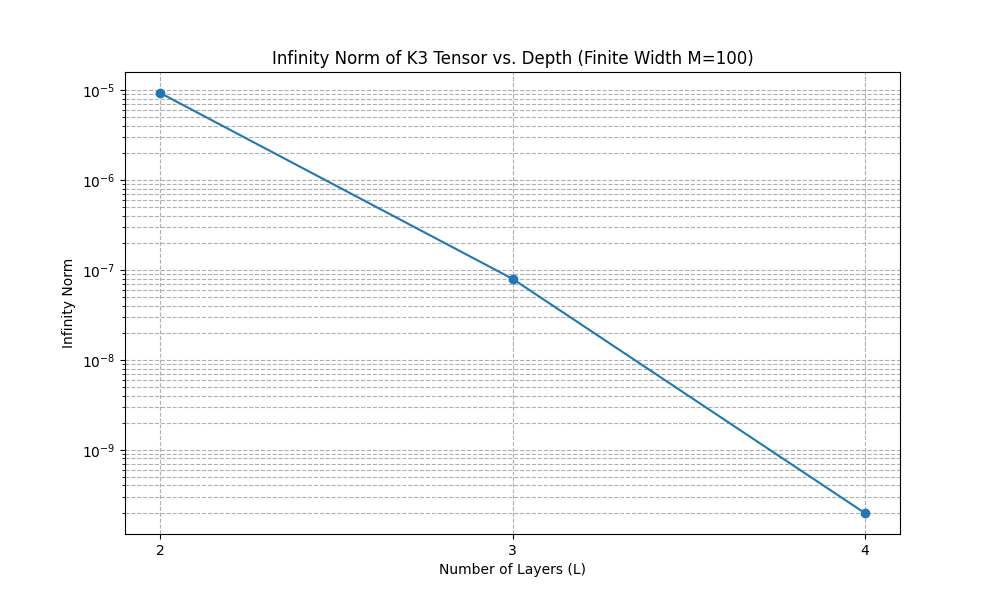
\includegraphics[width=0.8\textwidth]{../../../experiments/plots/k3_inf_norm_vs_L_finite_M100_N8_D20.png}
    \caption{Infinity norm of empirical $K^{(3)}$ vs. network depth $L$ (M=100).}
    \label{fig:k3_norm_vs_l}
\end{figure}
\begin{itemize}
    \item The plot clearly shows that the magnitude of $K^{(3)}$ \textbf{grows} with depth.
    \item The trend is strongly consistent with our theoretical prediction $K^{(3)} \sim \Order(L^2/\sqrt{m})$.
    \item This validates that finite-width effects become more pronounced in deeper networks.
\end{itemize}
\end{frame}


\section{Deeper Dive: NTK Correction Scaling}

\begin{frame}{Precise Scaling of the NTK Correction}
A multivariate regression in log-space ($R^2=0.994$) on the spectral radius of the correction $\|K - K_\infty\|$ yields a precise scaling law:

\begin{alertblock}{Empirical Scaling Law}
\[
\|K - K_\infty\| \propto L^{1.171} \cdot D_{\text{in}}^{0.047} \cdot N^{0.900} \cdot M^{-1.009}
\]
\end{alertblock}

\textbf{Interpretation:}
\begin{itemize}
    \item \textbf{Depth ($L$):} Super-linear growth.
    \item \textbf{Data Size ($N$):} Near-linear growth.
    \item \textbf{Input Dimension ($D_{in}$):} Essentially no dependence (good for high dimensions!).
    \item \textbf{Width ($M$):} Decays as $\sim 1/M$, as expected from theory.
\end{itemize}

\vfill
\tiny{\textit{Disclaimer: These results are based on extensive computations ($\sim$24h) and are fully reproducible via the provided codebase.}}

\end{frame}

\begin{frame}{Theoretical Interpretation}
The late-time correction $\Theta^{(1)}_\infty$ is given by a formula from \cite{large-width-feynman}:
\begin{align*}
\Theta^{(1)}_\infty \sim -\sum_{i}\frac{O_{3}}{\lambda_{i}} + \sum_{i,j}\frac{O_{4}}{\lambda_{i}(\lambda_{i}+\lambda_{j})}
\end{align*}

\textbf{Two key insights explain the scaling laws:}
\begin{enumerate}
    \item \textbf{Dominance of the $O_4$ Term:} The observed linear growth of the correction with depth $L$ suggests that the term involving the $O_4$ kernel is the primary driver of this behavior.
    \item \textbf{Role of $\lambda_{\min}$:} The correction terms are amplified by small eigenvalues $\lambda_i$. It is known that $\lambda_{\min} \sim \mathcal{O}(L/N)$.
    \begin{itemize}
        \item When $L$ increases or $N$ increases, $\lambda_{\min}$ gets smaller.
        \item This amplifies the correction, explaining the linear scaling with both $L$ and $N$.
    \end{itemize}
\end{enumerate}
\end{frame}


\section{Conclusion}

\begin{frame}{Conclusion}
\textbf{Summary:}
\begin{itemize}
    \item We moved beyond the infinite-width NTK by analyzing the NTH.
    \item We derived a complete formula for the first-order correction kernel, $K^{(3)}$.
    \item We showed theoretically and empirically that its magnitude scales as $\Order(H^2/\sqrt{m})$.
\end{itemize}
\vspace{1cm}
\textbf{Key Implication:}
\begin{alertblock}
The training dynamics of deep networks are inherently richer than shallow ones. The learning geometry itself (the NTK) evolves more significantly, meaning deep networks are less "lazy". This provides a theoretical basis for their powerful feature learning capabilities.
\end{alertblock}
\end{frame}

\end{document}
